\documentclass[a4paper]{article} 
\addtolength{\hoffset}{-2.25cm}
\addtolength{\textwidth}{4.5cm}
\addtolength{\voffset}{-3.25cm}
\addtolength{\textheight}{5cm}
\setlength{\parskip}{0pt}
\setlength{\parindent}{0in}

\usepackage[square,sort,comma,numbers]{natbib}
\usepackage{blindtext} % Package to generate dummy text
\usepackage{charter} % Use the Charter font
\usepackage[utf8]{inputenc} % Use UTF-8 encoding
\usepackage{microtype} % Slightly tweak font spacing for aesthetics
\usepackage{amsthm, amsmath, amssymb} % Mathematical typesetting
\usepackage{float} % Improved interface for floating objects
\usepackage{hyperref} % For hyperlinks in the PDF
\usepackage{graphicx, multicol} % Enhanced support for graphics
\usepackage{xcolor} % Driver-independent color extensions
\usepackage{pseudocode} % Environment for specifying algorithms in a natural way
\usepackage[mmddyy]{datetime} % Uses YEAR-MONTH-DAY format for dates

\usepackage{fancyhdr} % Headers and footers
\pagestyle{fancy} % All pages have headers and footers
\fancyhead{}\renewcommand{\headrulewidth}{0pt} % Blank out the default header
\fancyfoot[L]{} % Custom footer text
\fancyfoot[C]{} % Custom footer text
\fancyfoot[R]{\thepage} % Custom footer text
\newcommand{\note}[1]{\marginpar{\scriptsize \textcolor{red}{#1}}} % Enables comments in red on margin

\DeclareMathOperator*{\argmin}{arg\,min}

%----------------------------------------------------------------------------------------


%-------------------------------
%	TITLE VARIABLES (identify your work!)
%-------------------------------

\newcommand{\yourname}{Balthazar Neveu | Jamy Lafenetre}
\newcommand{\youremail}{balthazarneveu@gmail.com | jamy.lafenetre@ens-paris-saclay.fr}
\newcommand{\assignmentnumber}{3}

\begin{document}

%-------------------------------
%	TITLE SECTION (do not modify unless you really need to)
%-------------------------------
\fancyhead[C]{}
\hrule \medskip
\begin{minipage}{0.295\textwidth} 
\raggedright
\footnotesize
\yourname \hfill\\
\youremail
\end{minipage}
\begin{minipage}{0.4\textwidth} 
\centering 
\large 
Lab session \# \assignmentnumber\\ 
\normalsize 
NPM 2024\\ 
\end{minipage}
\begin{minipage}{0.295\textwidth} 
\raggedleft
\today\hfill\\
\end{minipage}
\medskip\hrule 
\bigskip




%-------------------------------
%	ASSIGNMENT CONTENT (add your responses)
%-------------------------------


\section*{Question 1}
\begin{figure}[ht]
  \centering
  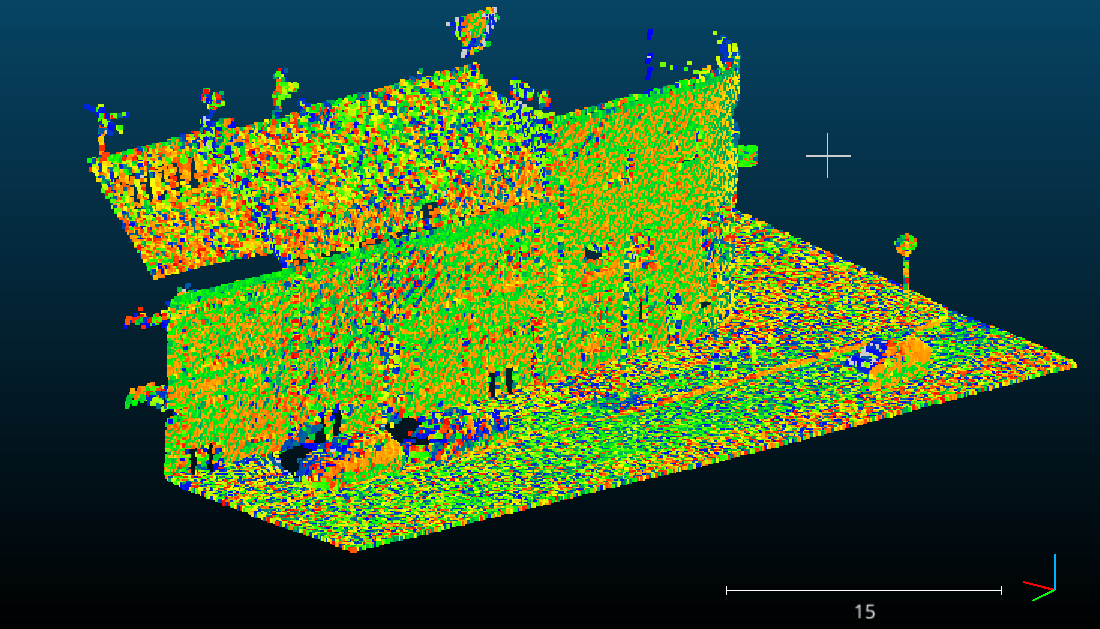
\includegraphics[width=0.3\linewidth]{figures/cc_normals_10cm.png}
  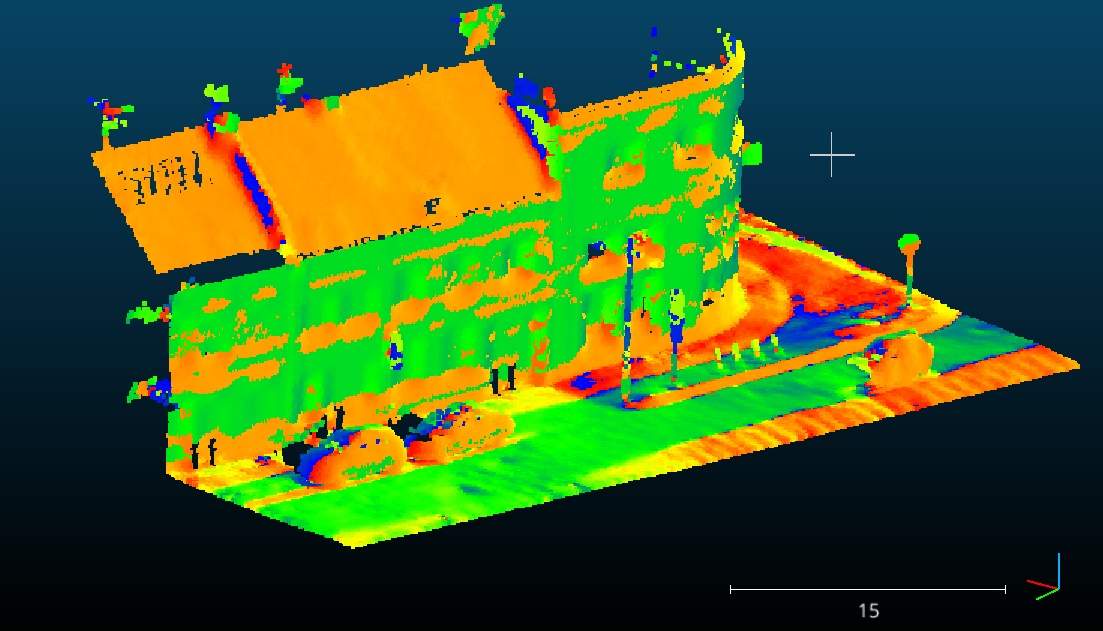
\includegraphics[width=0.3\linewidth]{figures/cc_normals_50cm.png}
  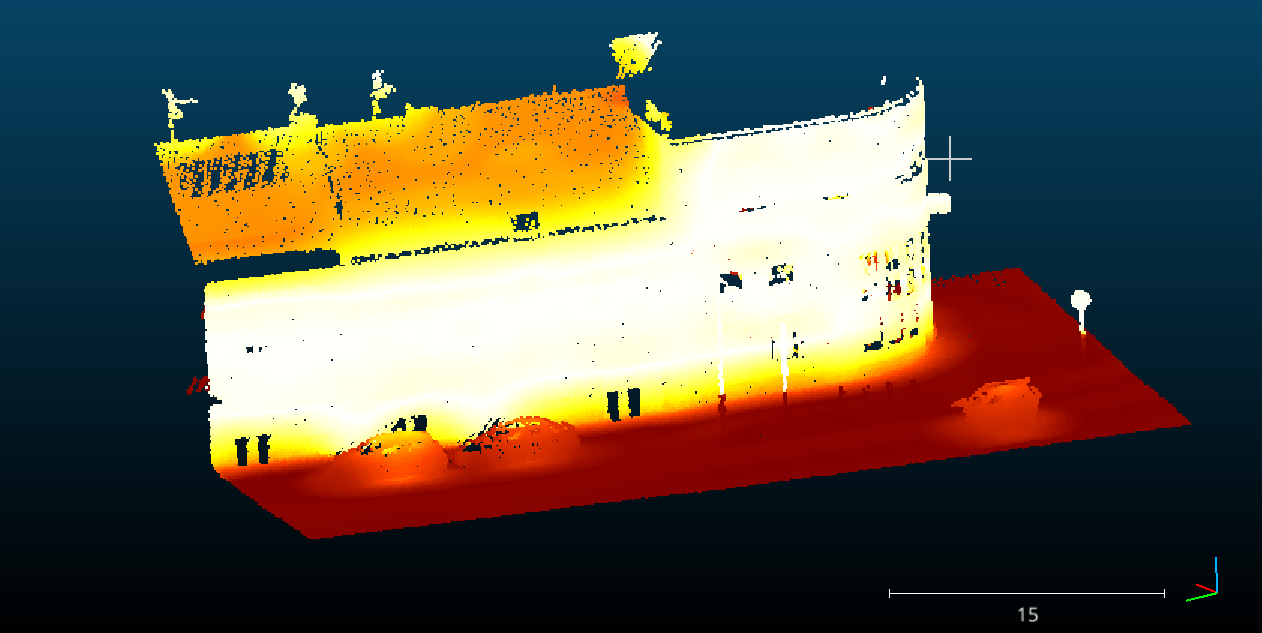
\includegraphics[width=0.3\linewidth]{figures/cc_normals_2m.png}
  
  \caption{From left to right: 10cm, 50cm, 2m radiuses used to compute normals}
  \label{fig:cc_normals}
\end{figure}
If the neighborhood radius is too small, we get noisy normals.
If the neighborhood radius is too large, we get smoothed normals (makes edges curvy).


\section*{Question 2}
Picking the right radius is a tradeoff between noisy normals and smoothing.


\section*{Question 3}
\begin{figure}[ht]
  \centering
  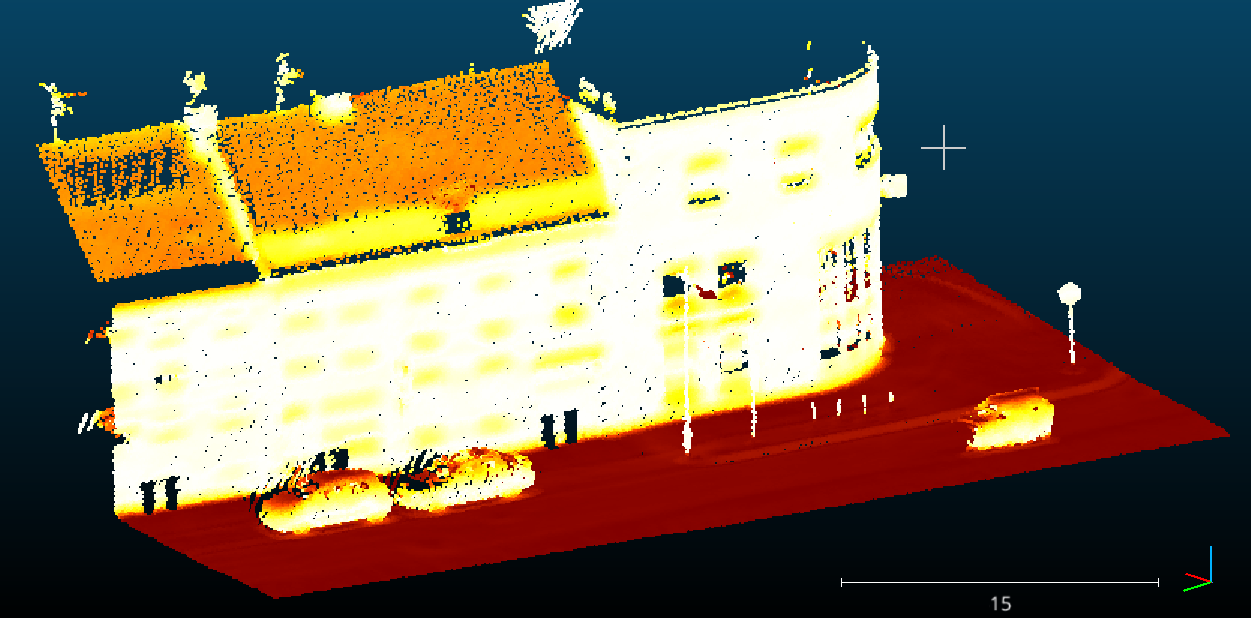
\includegraphics[width=.9\linewidth]{figures/cc_normals_PCA_50cm_bigger_points.png}
  \caption{50cm, radiuses local PCA used to compute normals}
  \label{fig:local_pca}
\end{figure}


\section*{Question 4}
\begin{figure}[ht]
  \centering
  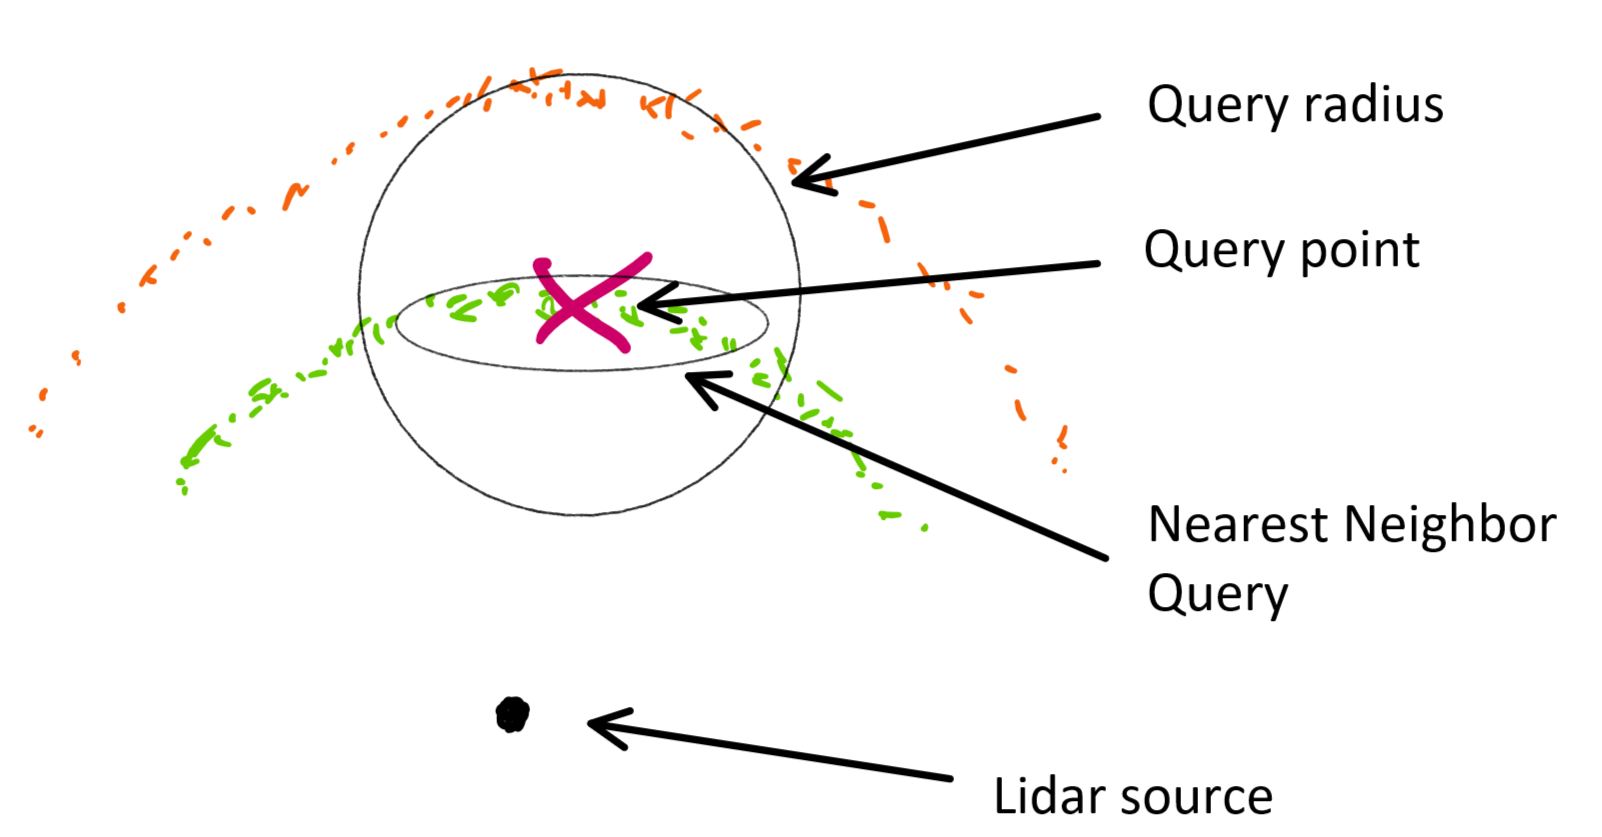
\includegraphics[width=.9\linewidth]{figures/Schema.png}
  \caption{Lidar acquisition leads to a specific points distribution. when combined with a fixed amount
  of nearest neighbors used to compute normals, this leads to visible artficats in the normal maps.
  } 
  \label{fig:lidar}
\end{figure}

The combination of lidar acquisition and the use of a fixed amount of nearest neighbors 
to compute normals leads to an anisotropic distribution of samples among each query.
Fitting a plane on such a set is not suited, a plane cannot be properly fitted with nearest neighbors.

The effect is also midly apparent when using a fixed radius because the radius may integrate other "beams" of the lidar.


\begin{figure}[ht]
  \centering
  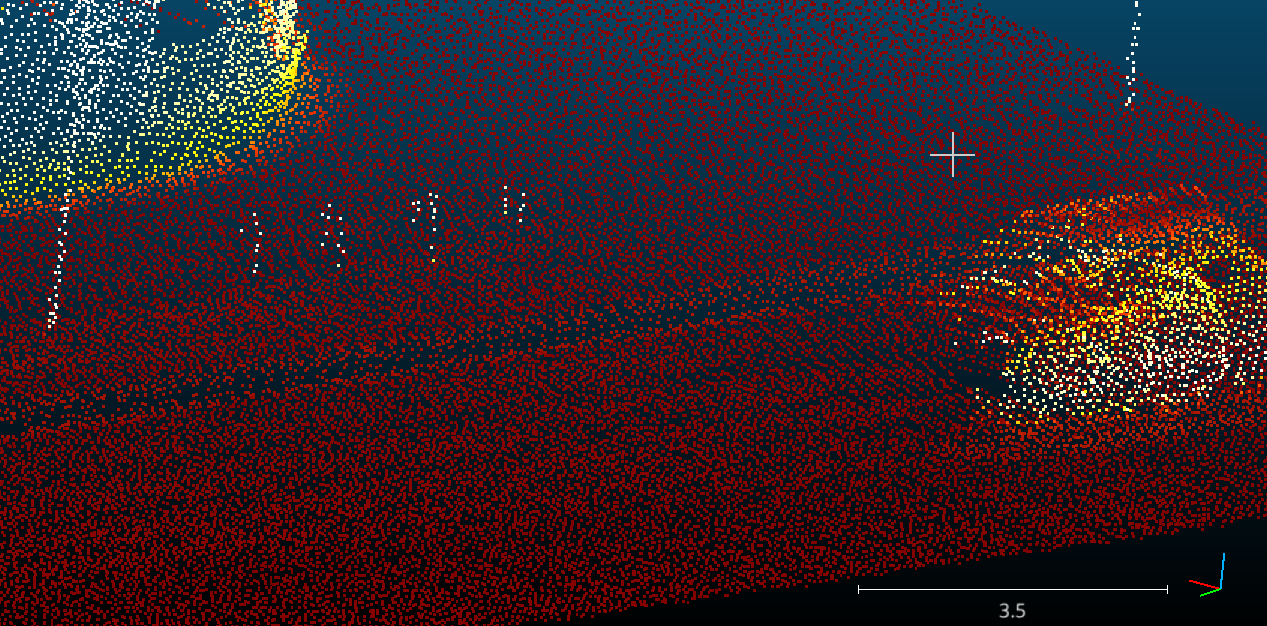
\includegraphics[width=0.46\linewidth]{figures/cc_normals_PCA_r=50cm_smooth.png}
  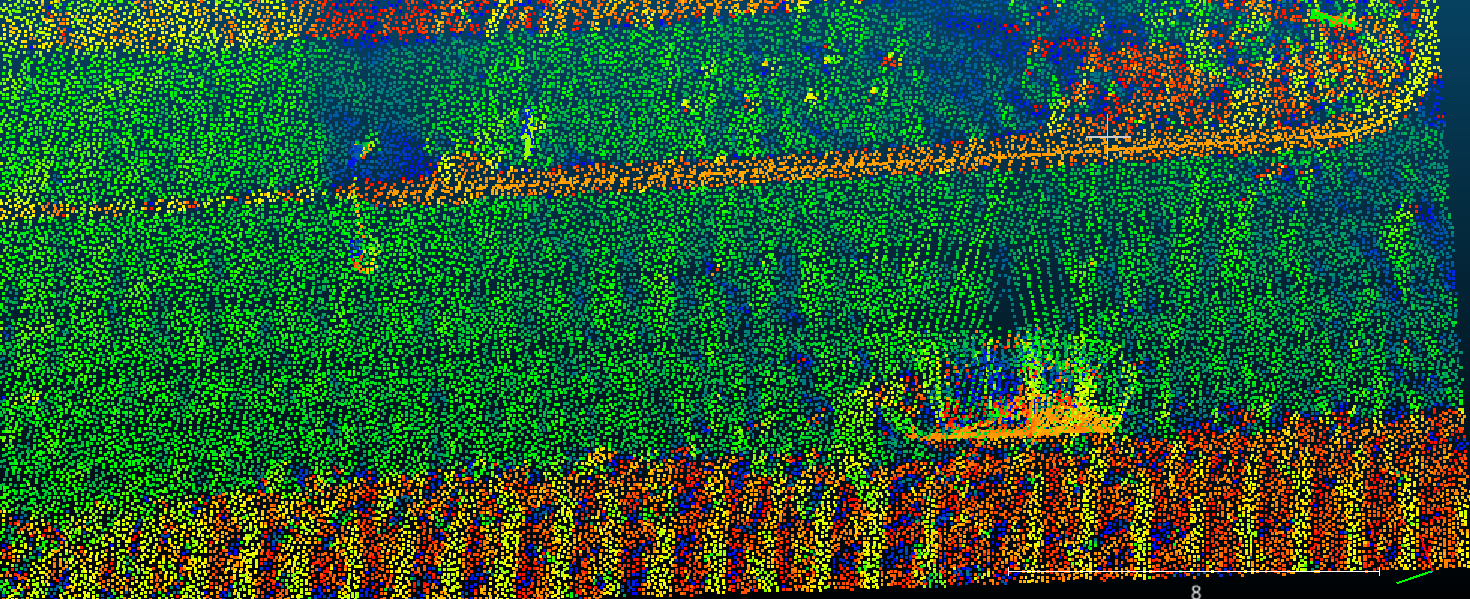
\includegraphics[width=0.46\linewidth]{figures/cc_normals_PCA_50cm_k=30_nearest.png}
  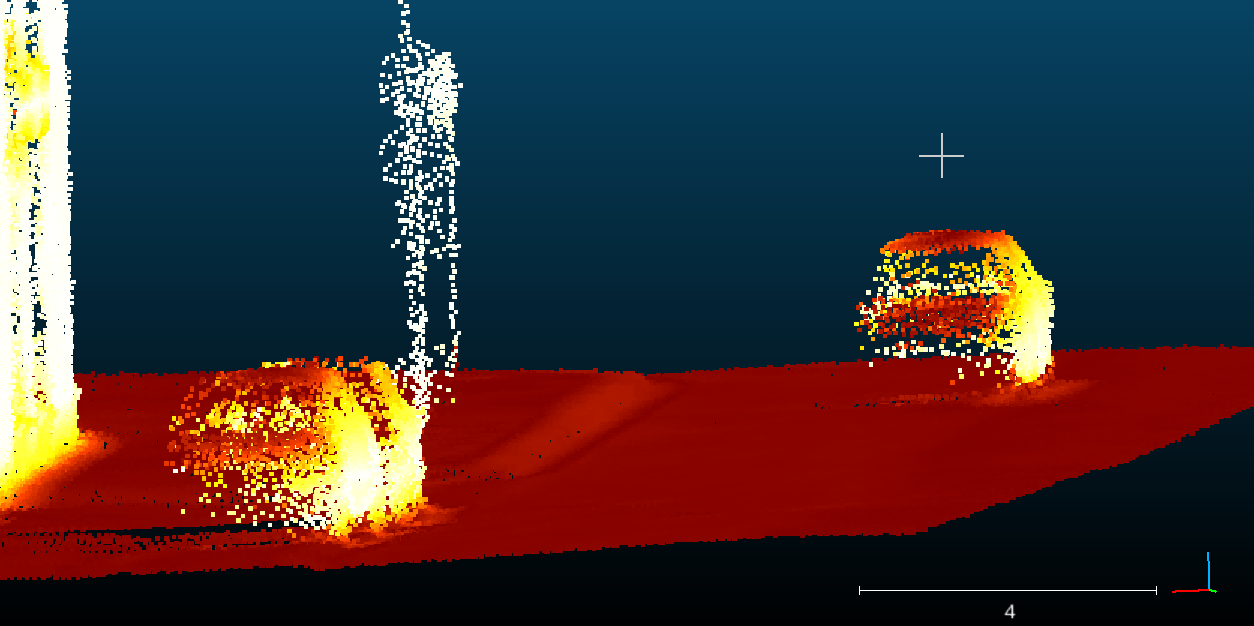
\includegraphics[width=0.46\linewidth]{figures/cc_normals_PCA_r=50cm_v2.png}
  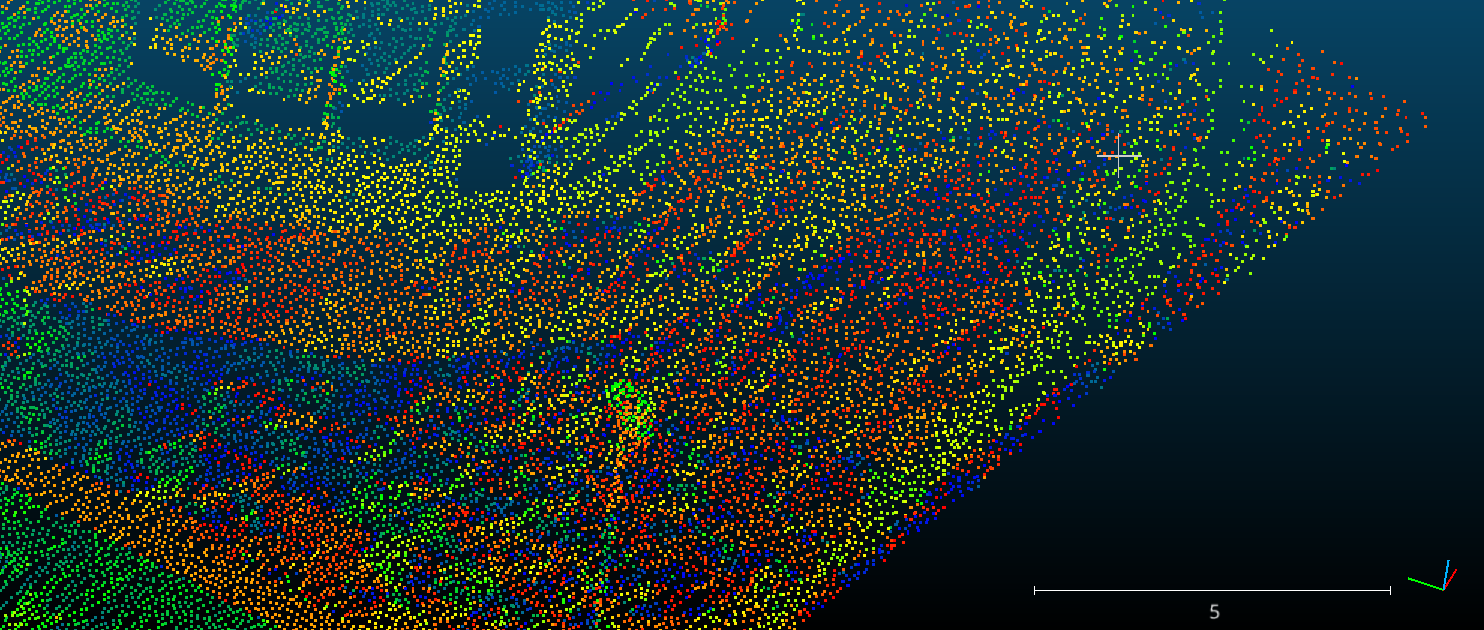
\includegraphics[width=0.46\linewidth]{figures/cc_normals_PCA_50cm_k=30_v2.png}
  \caption{Left: 50cm radius local PCA used to compute normals. 
  Right: 30 nearest neighbors used to compute normals.} 
  \label{fig:local_PCA_neighbor}
\end{figure}


\end{document}

